\documentclass[aspectratio=169, french]{beamer}
\usepackage{fontspec}
\usepackage[french]{babel}
\usefonttheme{professionalfonts}
\usepackage{amsmath,amssymb,amsthm}
\usepackage{arydshln,mathtools}
\usepackage{bm}
\usepackage{color}
\definecolor{theme}{RGB}{0,73,114}
\usepackage{multicol}
%\usepackage[caption=false]{subfig}
\usepackage{subcaption}

\usepackage{comment}

\usepackage{graphicx}
\usepackage{diffcoeff}
\usepackage{dsfont}
\usepackage{mathrsfs}
\usepackage[most]{tcolorbox}

\usepackage{xspace}
\usepackage{appendixnumberbeamer}


\usepackage{media9}
\usepackage[backend=bibtex, style=verbose]{biblatex}
\bibliography{biblioTrEquation}
%\renewcommand\bibfont{\scriptsize}

\addtobeamertemplate{footnote}{\vspace{-6pt}\advance\hsize-0.5cm}{\vspace{6pt}}
\makeatletter
% Alternative A: footnote rule
\renewcommand*{\footnoterule}{\kern -3pt \hrule \@width 2in \kern 8.6pt}
% Alternative B: no footnote rule
% \renewcommand*{\footnoterule}{\kern 6pt}
\makeatother

\graphicspath{{./images/}}



% Math macros
\DeclareMathOperator*{\grad}{grad}
\DeclareMathOperator*{\Grad}{Grad}
\DeclareMathOperator*{\Div}{Div}
\renewcommand{\div}{\operatorname{div}}
\DeclareMathOperator*{\Hess}{Hess}
\DeclareMathOperator*{\curl}{curl}
\DeclareMathOperator{\Tr}{Tr}
\DeclareMathOperator{\Dom}{Dom}
\DeclareMathOperator*{\esssup}{ess\,sup}

\newcommand{\bbR}{\mathbb{R}}
\newcommand{\bbC}{\mathbb{C}}
\newcommand{\bbF}{\mathbb{F}}
\newcommand{\bbA}{\mathbb{A}}
\newcommand{\bbB}{\mathbb{B}}
\newcommand{\bbS}{\mathbb{S}}

\newcommand*{\norm}[1]{\ensuremath{\left\|#1\right\|}}
\newcommand{\where}{\qquad \text{where} \qquad}
\newcommand{\inner}[3][]{\ensuremath{\left\langle #2, \, #3 \right\rangle_{#1}}}
\newcommand{\bilprod}[2]{\left\langle \left\langle \, #1, #2 \, \right\rangle \right\rangle}
\newcommand{\pder}[2]{\ensuremath{\partial_{#2} #1}}
\newcommand{\dder}[2]{\ensuremath{\delta_{#2} #1}}
\newcommand{\secref}[1]{\S\ref{#1}}
\newcommand{\energy}[1]{\frac{1}{2} \int_{\Omega} \left\{ #1 \right\} \d\Omega}
\newcommand{\crmat}[1]{\ensuremath{\left[#1\right]_\times}}
\newcommand{\fenics}{\textsc{FEniCS}\xspace}
\newcommand{\firedrake}{\textsc{Firedrake}\xspace}

\DeclareMathOperator*{\argmax}{arg\,max}
\DeclareMathOperator*{\argmin}{arg\,min}

\newtheorem{proposition}{Proposition}
\newtheorem{remark}{Remark}
\newtheorem{hypothesis}{Hypothesis}
\newtheorem{assumption}{Assumption}
\newtheorem{conjecture}{Conjecture}


\def\onedot{$\mathsurround0pt\ldotp$}
\def\cddot{% two dots stacked vertically
	\mathbin{\vcenter{\baselineskip.67ex
			\hbox{\onedot}\hbox{\onedot}}%
}}


\setbeamertemplate{blocks}[rounded][shadow]

\setbeamercolor{block body alerted}{bg=alerted text.fg!10}
\setbeamercolor{block title alerted}{bg=alerted text.fg!20}
\setbeamercolor{block body}{bg=structure!10}
\setbeamercolor{block title}{bg=structure!20}
\setbeamercolor{block body example}{bg=green!10}
\setbeamercolor{block title example}{bg=green!20}

% Remove navigation bar
\setbeamertemplate{navigation symbols}{}


\makeatletter \renewcommand\d[1]{\ensuremath{%
		\;\mathrm{d}#1\@ifnextchar\d{\!}{}}}
\makeatother


\graphicspath{{./imagesEqTr/}}

\newif\iftocsub
\tocsubtrue
\AtBeginSection[] {
	\begin{frame}[noframenumbering]{Outline}
		\tableofcontents[sectionstyle=show/shaded, subsectionstyle=show/show/hide]
	\end{frame}
	\tocsubfalse
}
\AtBeginSubsection[] {
	\iftocsub
	\begin{frame}[noframenumbering]{Outline}
		\tableofcontents[currentsubsection, sectionstyle=show/shaded, subsectionstyle=show/shaded/hide]
	\end{frame}
	\fi
	\tocsubtrue
}

\newcommand{\beginbackup}{
	\newcounter{framenumbervorappendix}
	\setcounter{framenumbervorappendix}{\value{framenumber}}
}
\newcommand{\backupend}{
	\addtocounter{framenumbervorappendix}{-\value{framenumber}}
	\addtocounter{framenumber}{\value{framenumbervorappendix}} 
}


\begin{document}
	
	
\begin{frame}[plain]
	
	%%%%%%%% Title slide details %%%%%%%%%%%%%%


% Background Image
\newcommand{\myBackground}
{
    
\includegraphics[height=1.02\paperheight,page=9]{beamerthemeutresources}
}

% Title
\newcommand{\myTitle}
{
Méthodes des différences finies
}

% Subtitle
\newcommand{\mySubTitle}
{
EDP de transport 1D
}

% Author
\newcommand{\myAuthor}   
{
    Andrea Brugnoli
}

% Affiliation
\newcommand{\myAffiliate}
{
  
}

% Presentation Date
\newcommand{\myDate}   
{
    11 Avril 2022
}

% Logo
\newcommand{\myLogo}   
{
    
\includegraphics[width=3cm]{Logo.png}
}
%%%%%%%%%%%%%%%%%%%%%%%%%%%%%%%%%%%%


%%%%%%%%%% Title slide code %%%%%%%%%%%
\begin{tikzpicture}[remember picture,overlay]

% Background color

\fill[white] (current page.south west) rectangle (current page.north east);
% Background image
\node[above right,inner sep=0pt] at (current page.south west)
    {
        \myBackground
    };
    
% Title & Subtitle
\node
[
    above=0.5cm,
    align=center,
    draw=black!50,
    % rounded corners,
    double,
    double distance=0.1cm,
    double=blue!10,
    fill=theme!10,
    inner xsep=15pt,
    inner ysep=10pt, 
    minimum width=0.8\textwidth,
    text width=0.8\textwidth
] (title) at (current page.center)
{
    \LARGE \myTitle  \\[5pt]
    \small \mySubTitle
};

% Author 
\node[ below=0.5cm] (author) at (title.south){\myAuthor};

% Author 
\node[ below=0.25cm ](affiliate) at (author.south){\small \myAffiliate};

% Date
\node[below=0.25] (date) at (affiliate.south){\large \myDate};

% Logo
\node
[
    below =0.25cm
] at (date.south)
{
    \myLogo
};

\end{tikzpicture}
	
\end{frame}
	
	
\begin{frame}{Aperçu}
	
	\tableofcontents
	
\end{frame}

\section{Équation du transport 1D : le cas continu}

\begin{frame}{Équation du transport 1D}
	\begin{tcolorbox}[title = L'EDP la plus simple, coltitle=white]
		L'évolution d'un champ scalaire $u(x, t)$ transporté par un fluide satisfait 
		\begin{equation*}
			\diffp{u}{t} + \diffp{q}{x} = 0, \qquad x \in \bbR, \quad t \in  (0, T]. 
		\end{equation*}
	\end{tcolorbox}

\begin{tcolorbox}
	Pour le flux $q(u, x, t)$ on considère une vitesse constante pour le fluide
	\begin{equation*}
		q(u, x, t) = c \, u(x, t), \qquad c \in \bbR.
	\end{equation*}
	Le problème est bien posé lorsque on spécifie la donnée initiale
	\begin{align*}
		u(x, 0) &= u_0(x). 
	\end{align*}
\end{tcolorbox}

\end{frame}

\begin{frame}{Solution Analytique}
	\begin{columns}
	\begin{column}{.58\textwidth}
		\begin{overlayarea}{\textwidth}{\textheight}
		\vspace{1cm}
		\begin{tcolorbox}[title = Solution analytique regulière, coltitle=white]
			Si $u_0 \in C^{1}(\bbR)$ alors  
			$u \in C^{1}(\bbR \times[0, T])$ et
			\begin{equation*}
				u(x, t) = 	u_0(x - ct),
			\end{equation*}
		i.e. $u$ constant sur $\gamma$ telle que $\dot{\gamma} = (c ,1)$. \\
		Les courbes $\gamma$ sont appelées caractéristiques.
		\end{tcolorbox}
		\end{overlayarea}
	\end{column}
	\begin{column}{.42\textwidth}
		\begin{overlayarea}{\textwidth}{\textheight}
		\begin{figure}[t]
			\only<1>{\includegraphics[height=.75\textheight]{u_sol_c_pos_nobcs.eps}%
				\caption*{Exemple : $u_0(x) = e^{-x^2/4}, \; c>0$.}
			}
			\only<2>{
				\includegraphics[height=.75\textheight]{u_sol_c_neg_nobcs.eps} 
				\caption*{Exemple : $u_0(x) = e^{-x^2/4}, \; c<0$.}
			}
		\end{figure}
		\end{overlayarea}
	\end{column}
\end{columns}


\end{frame}

\section{Discrétisation par différence finies}

\subsection{Maillage et approximation des dérivées}

\begin{frame}{Discrétisation du domaine : le maillage}
On considère un maillage rectangulaire uniforme $(x_i, t_n)$ : \\
cela signifie que $\Delta x = x_{i+1}- x_i $ et $\Delta t = t_{n+1}- t_n$ sont constants. \\
  

	\begin{columns}
	\begin{column}{.5\textwidth}
	\begin{figure}
		\includegraphics[height=.5\textheight]{mesh.eps}
		\caption*{Exemple de maillage rectangulaire uniforme :\\ $\Delta x = 4, \quad \Delta t=2$.}
	\end{figure}	
	\end{column}
	\begin{column}{.5\textwidth}
		\begin{tcolorbox}
			La solution discrète $u_{i, n}$ au n\oe{}ud $(x_i, t_n)$ est une approximation  de la valeur exacte $u(x_i, t_n)$
			\begin{equation*}
				u_{i, n} \approx u(x_i, t_n).
			\end{equation*} 
		\end{tcolorbox}
	\end{column}
\end{columns}	

\end{frame}


\begin{frame}{Approximation des dérivées : développement de Taylor}
	\textbf{Différences finies : on remplace la dérivée par un quotient différentiel}
	
	
	\begin{columns}
		\begin{column}{.5\textwidth}
			\begin{tcolorbox}[title=Discrétisation en temps, coltitle=white]
				Explicite
				\begin{equation*}
					\begin{aligned}
						\diffp{u}{t}(x_i, t_n) \approx \frac{u_{i, n+1} - u_{i, n}}{\Delta t} + O(\Delta t).
					\end{aligned}
				\end{equation*}
				Implicite
				\begin{equation*}
					\begin{aligned}
						\diffp{u}{t}(x_i, t_n) \approx \frac{u_{i, n} - u_{i, n-1}}{\Delta t} + O(\Delta t).
					\end{aligned}
				\end{equation*}
				Centrée
				\begin{equation*}
					\begin{aligned}
						\diffp{u}{t}(x_i, t_n) \approx \frac{u_{i, n+1} - u_{i, n-1}}{2\Delta t} + O(\Delta t^2)
					\end{aligned}
				\end{equation*}
			\end{tcolorbox}
		\end{column}
		\begin{column}{.5\textwidth}
			\begin{tcolorbox}[title=Discrétisation en espace, coltitle=white]
				Aval
				\begin{equation*}
					\diffp{u}{x}(x_i, t_n) \approx \frac{u_{i+1, n} - u_{i, n}}{\Delta x} + O(\Delta x).
				\end{equation*}
				Amont
				\begin{equation*}
					\diffp{u}{x}(x_i, t_n) \approx \frac{u_{i, n} - u_{i-1, n}}{\Delta x} + O(\Delta x).
				\end{equation*}
				Centrée
				\begin{equation*}
					\diffp{u}{t}(x_i, t_n) \approx \frac{u_{i+1, n} - u_{i-1, n}}{2\Delta x} + O(\Delta x^2)
				\end{equation*}
			\end{tcolorbox}
			\end{column}
		\end{columns}	
	
	
\end{frame}


\subsection{Stabilité : analyse de Von Neumann}


\begin{frame}{Quoi choisir? Analyse de Von Neumann}
	\textbf{Intuition : } Solution de l'EDP de transport pour $u_0(x) = e^{j \xi x} \; (j = \sqrt{-1})$ :
	\begin{equation*}
	u(x, t) = e^{j \xi(x-ct)} = e^{j \xi x}e^{-jct}, \qquad \text{Onde plane.}
	\end{equation*}
	\textbf{Justification (analyse de Fourier)} :  la transformé de Fourier de $u(x, \cdot)$ est
	\begin{equation*}
		\widehat{u}(\xi, \cdot) = \mathcal{F}\{u\}(\xi, \cdot) = \int_{-\infty}^{+\infty} u(x, \cdot)e^{- j \xi x}  \d{x}, \qquad \xi \in \bbR.
	\end{equation*}

La transformé de la dérivée est donnée par
\begin{equation*}
\mathcal{F}\{\partial_{x} u\}(\xi, \cdot) = j \xi \widehat{u}(\xi, \cdot).
\end{equation*}
EDP du transport : $\partial_t{\widehat{u}}(\xi, t) = -c  j  \xi \widehat{u}(\xi, t)$ \hspace{.3cm} (Eq. algébrique in $\bbC$).
\begin{block}{Analyse de von Neumann : un outils simple mais très efficace}
		On considère alors l'évolution en temps discret du mode
		\begin{equation*}
			u_{i, n} = \psi_n e^{\, j \xi  i  \Delta x}, \quad \psi_n \in \bbC.
		\end{equation*}
\end{block}
\end{frame}

\begin{frame}{Rappel : stabilité des systèmes dynamiques discrets}
	\begin{columns}
		\begin{column}{.55\textwidth}
			\begin{block}{Stabilité en temps discret (cas complexe)}
				Le système discret temps invariant
				\begin{equation*}
					\begin{aligned}
						\psi_{n+1} &= A \psi_n, \qquad \psi_n \in \mathbb{C},  \; A \in \mathbb{C},\\
						\psi_0 &= \overline{\psi},
					\end{aligned}
				\end{equation*}  
				est stable si $|A|<1$ et stable au sens de Lyapunov si $|A|=1$.
			\end{block}
		\end{column}
		\begin{column}{.45\textwidth}
			\begin{figure}
				\centering
				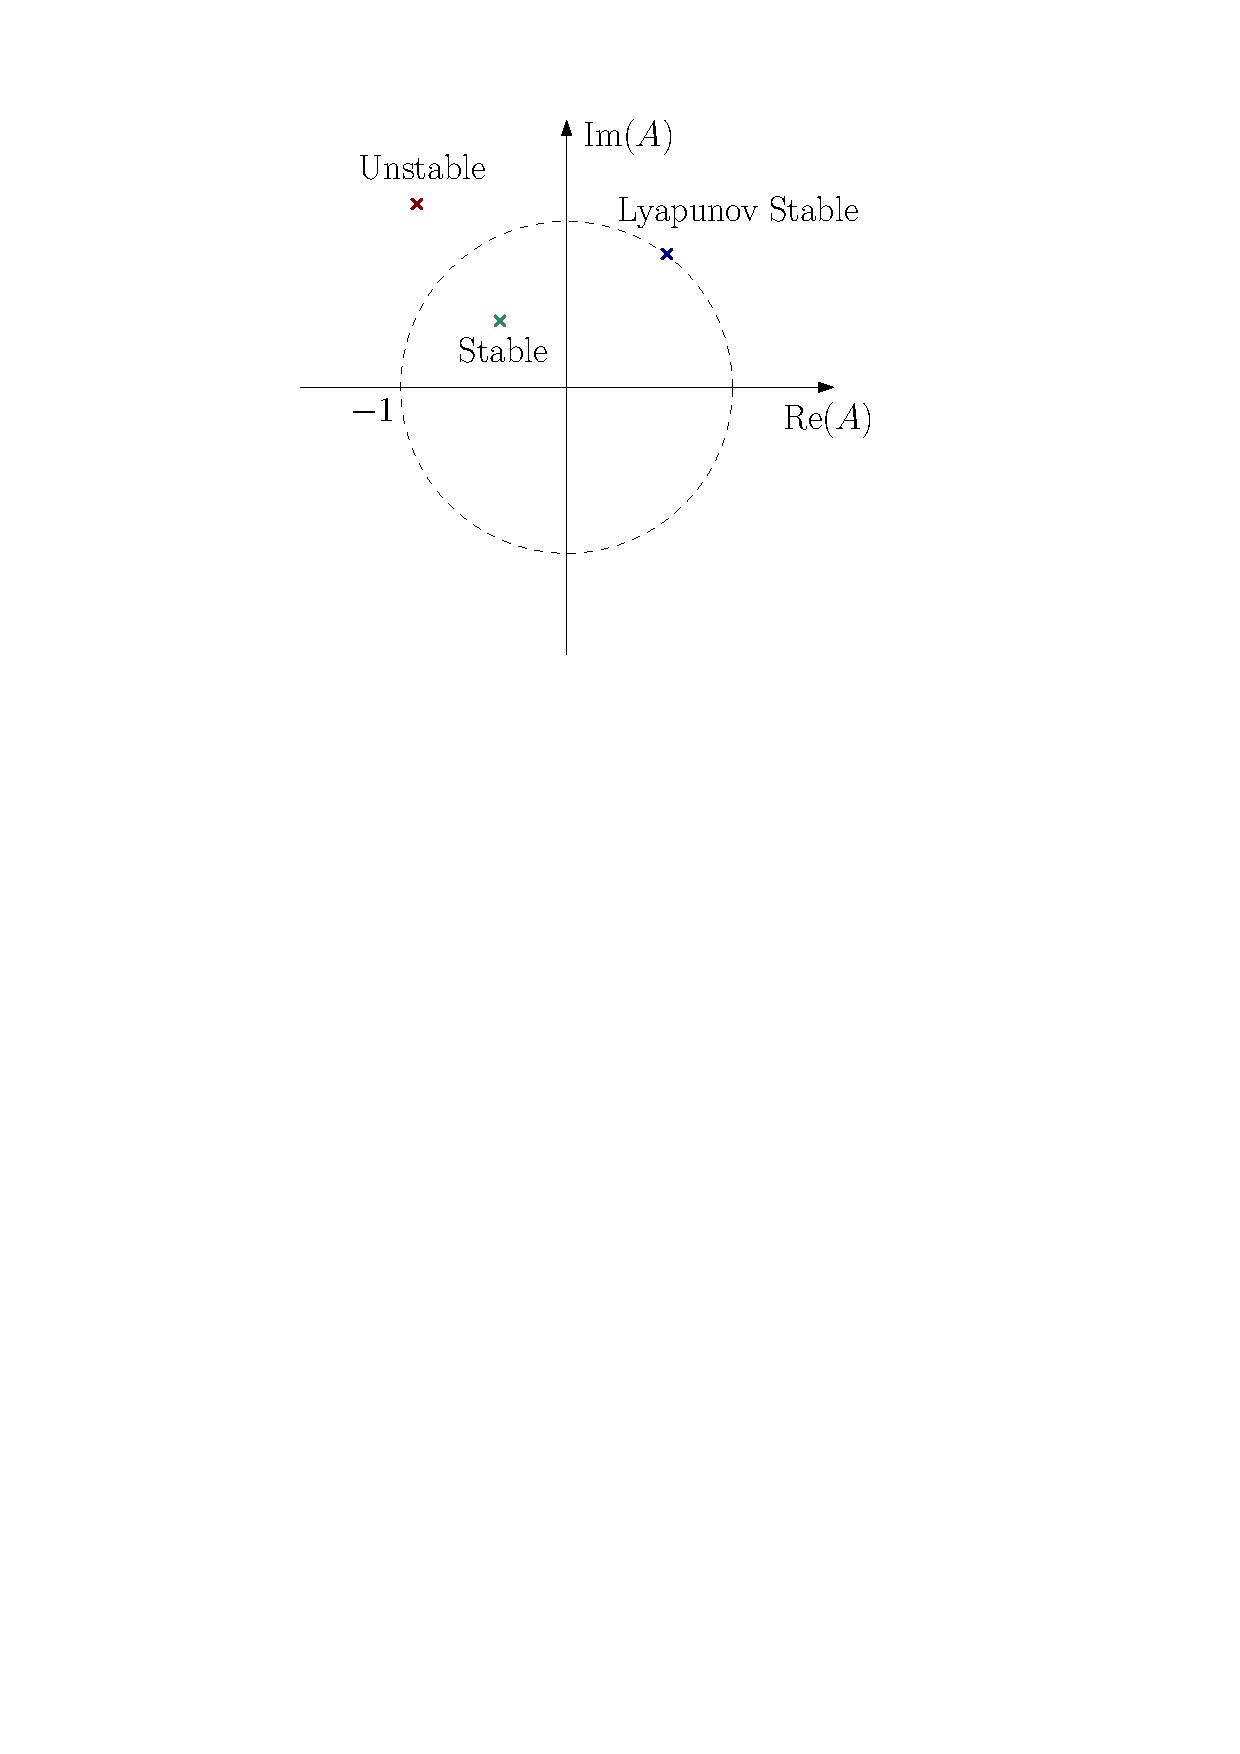
\includegraphics[height=.7\textheight]{discrete_stability.pdf}
			\end{figure}
		\end{column}
	\end{columns}	
\end{frame}

\subsection{Applications}

\begin{frame}{Les schémas que on va analyser}
\begin{enumerate}
	\item Explicite en temps, aval en espace.
	\item Explicite en temps, amont en espace.
	\item Explicite en temps, centré en espace.
	\item Implicite en temps, amont en espace.
\end{enumerate} 
\end{frame}


\begin{frame}{Cas 1 : Schéma explicite en temps et aval en espace}
Schéma résultant : 
$u_{i, n+1} = u_{i, n} - \sigma(u_{i+1, n} - u_{i, n})$ \\
où $\sigma = c/c_{\mathrm{num}}$. ($c_{\mathrm{num}} = \Delta x/\Delta t$ est la \textbf{vitesse numérique})

\begin{tcolorbox}
L'hypothèse du Von Neumann $u_{i, n} = \psi_n e^{\, j  \xi  i  \Delta x}$ donne $\psi_{n+1} = A(\xi) \psi_n$ où
\begin{equation*}
	A(\xi) = 1 - \sigma(e^{j  \xi \Delta x}-1), \qquad \text{Coefficient d'amplification}.
\end{equation*}
Le critère de stabilité est respecté si
\begin{equation*}
	|A(\xi)|^2 = 1 + 2 \sigma(\sigma + 1)(1 - \cos(\xi \Delta x))\le 1 \implies \textbf{Stable si}   -1 \le \sigma \le 0
\end{equation*}
Si $\sigma=-1 \implies |A(\xi)|=1$ (pas de viscosité numérique)\\
Si $-1 < \sigma \le 0 \implies |A(\xi)|<1$ (viscosité numérique)
\begin{equation*}
	\begin{aligned}
	c<0, \\
	c_{\mathrm{num}}>|c|, 
	\end{aligned}
	\qquad 
	\begin{aligned}
	\text{Discrétisation aval ne peut pas traiter vitesse postive}, \\
	\text{Condition CFL (Courant, Friedrichs et Lewy 1928).}
	\end{aligned}
\end{equation*}

\end{tcolorbox}

\end{frame}



\begin{frame}{Résultats simulation}
	
\only<1>{
\centering
\includemedia[
label=vidcas1_sig_m1,
addresource=/home/andrea/Videos/PresEqTransport/cas1_sig_m1.mp4,
activate=pageopen, 
deactivate=onclick,
width=.8\textwidth, height=.7\textheight,
flashvars={
	source=/home/andrea/Videos/PresEqTransport/cas1_sig_m1.mp4
	&%
	autoPlay=true&%
	loop=true%
}
]{}{VPlayer.swf}
Cas stable sans viscosité numérique.
%\mediabutton[
%mediacommand=vidPlateRod:playPause
%]{\fbox{Play/Pause}}
}

	
\only<1>{
	\centering
	\includemedia[
	label=vidcas1_sig_mdot5,
	addresource=/home/andrea/Videos/PresEqTransport/cas1_sig_mdot5.mp4,
	activate=pageopen, 
	deactivate=onclick,
	width=.8\textwidth, height=.7\textheight,
	flashvars={
		source=/home/andrea/Videos/PresEqTransport/cas1_sig_mdot5.mp4
		&%
		autoPlay=true&%
		loop=true%
	}
	]{}{VPlayer.swf}
	Cas stable avec viscosité numérique.
	%\mediabutton[
	%mediacommand=vidPlateRod:playPause
	%]{\fbox{Play/Pause}}
}

	
\only<1>{
	\centering
	\includemedia[
	label=vidcas1_sig_m2,
	addresource=/home/andrea/Videos/PresEqTransport/cas1_sig_m2.mp4,
	activate=pageopen, 
	deactivate=onclick,
	width=.8\textwidth, height=.7\textheight,
	flashvars={
		source=/home/andrea/Videos/PresEqTransport/cas1_sig_m2.mp4
		&%
		autoPlay=true&%
		loop=true%
	}
	]{}{VPlayer.swf}
	Instable : CFL non respectée.
	%\mediabutton[
	%mediacommand=vidPlateRod:playPause
	%]{\fbox{Play/Pause}}
}

	
\only<4>{
	\centering
	\includemedia[
	label=vidcas1_sig_dot5,
	addresource=/home/andrea/Videos/PresEqTransport/cas1_sig_dot5.mp4,
	activate=pageopen, 
	deactivate=onclick,
	width=.8\textwidth, height=.7\textheight,
	flashvars={
		source=/home/andrea/Videos/PresEqTransport/cas1_sig_dot5.mp4
		&%
		autoPlay=true&%
		loop=true%
	}
	]{}{VPlayer.swf}
	Cas instable (c>0).
	%\mediabutton[
	%mediacommand=vidPlateRod:playPause
	%]{\fbox{Play/Pause}}
}

\end{frame}




\section{Pour aller plus loin : domaine borné et conditions au bord}

\begin{frame}{Domaine borné en espace}
	
On considère le transport du champ $u(x, t)$ dans un domaine spatial borné
\begin{equation*}
	\diffp{u}{t} + c \diffp{u}{x} = 0, \qquad c > 0, \quad  x \in [0, L], \quad t \in (0, T]. 
\end{equation*}
		
		Le problème est bien posé lorsque on spécifie 
		\begin{equation*}
			\begin{aligned}
			u(x, 0) &= u_0(x),\\
			u(0, t) &= f(t),
			\end{aligned} \qquad
			\begin{aligned}
			\text{Donnée initiale}, \\
			\text{Condition au bord}.
			\end{aligned}
		\end{equation*}
	\begin{tcolorbox}[title = Solution analytique, coltitle=white]
Si $f, \; u_0 \in C^{1}$, et $f(0) = u_0(0), \; f^{'}(0) = -c u_0{'}(0)$
alors  $u \in C^{1}([0, L]\times [0, T])$ 
\begin{equation*}
	u(x, t) = \begin{cases}
		u_0(x - ct), \quad &x\ge ct\\
		f(t-x/c), \quad &x\le ct,
	\end{cases}
	\qquad\text{i.e. $u$ constant sur $\gamma$ telle que $\dot{\gamma} = (c ,1)$.}
\end{equation*}
\end{tcolorbox}
	
\end{frame}

\begin{frame}{Compatibilité de données}

	\begin{columns}
		\begin{column}{.5\textwidth}
			\begin{overlayarea}{\textwidth}{\textheight}
			\begin{block}{Interaction entre les données}
				\begin{equation*}
					u(x, t) = 
					\begin{cases}
						u_0(x - ct), \quad &x\ge ct\\
						f(t-x/c), \quad &x\le ct,
					\end{cases}
				\end{equation*}
				$f$ et $u_0$ interagissent seulement sur $x=ct$.
			\end{block}
				\begin{tcolorbox}[title = Exemples, coltitle=white]
					$c=2, \quad L=20, \quad T = 10$.
					\begin{align*}
						u_0(x) &= e^{-x^2/4}, \\
						f(t) &= \only<1>{1,}  \only<2>{e^{-t^2},}  \only<3>{\cos^2(t),}
					\end{align*}
				\end{tcolorbox}	
			\end{overlayarea}
		\end{column}
		\begin{column}{.5\textwidth}
		\begin{overlayarea}{\textwidth}{\textheight}
			\begin{figure}
				\centering
				\only<1>{\includegraphics[height=.8\textheight]{u_sol_f1.eps}}
				\only<2>{\includegraphics[height=.8\textheight]{u_sol_f2.eps}}			
				\only<3>{\includegraphics[height=.8\textheight]{u_sol_f3.eps}}
			\end{figure}
		\end{overlayarea}
		\end{column}
	\end{columns}	

\end{frame}


\begin{frame}{Bibliographie}
	%\bibliographystyle{unsrt}
	\nocite{*}
	\printbibliography
\end{frame}
	
	
\end{document}